\label{ch:appendix}
\section{16-17th night} 

\begin{figure}[!ht]
    \centering
    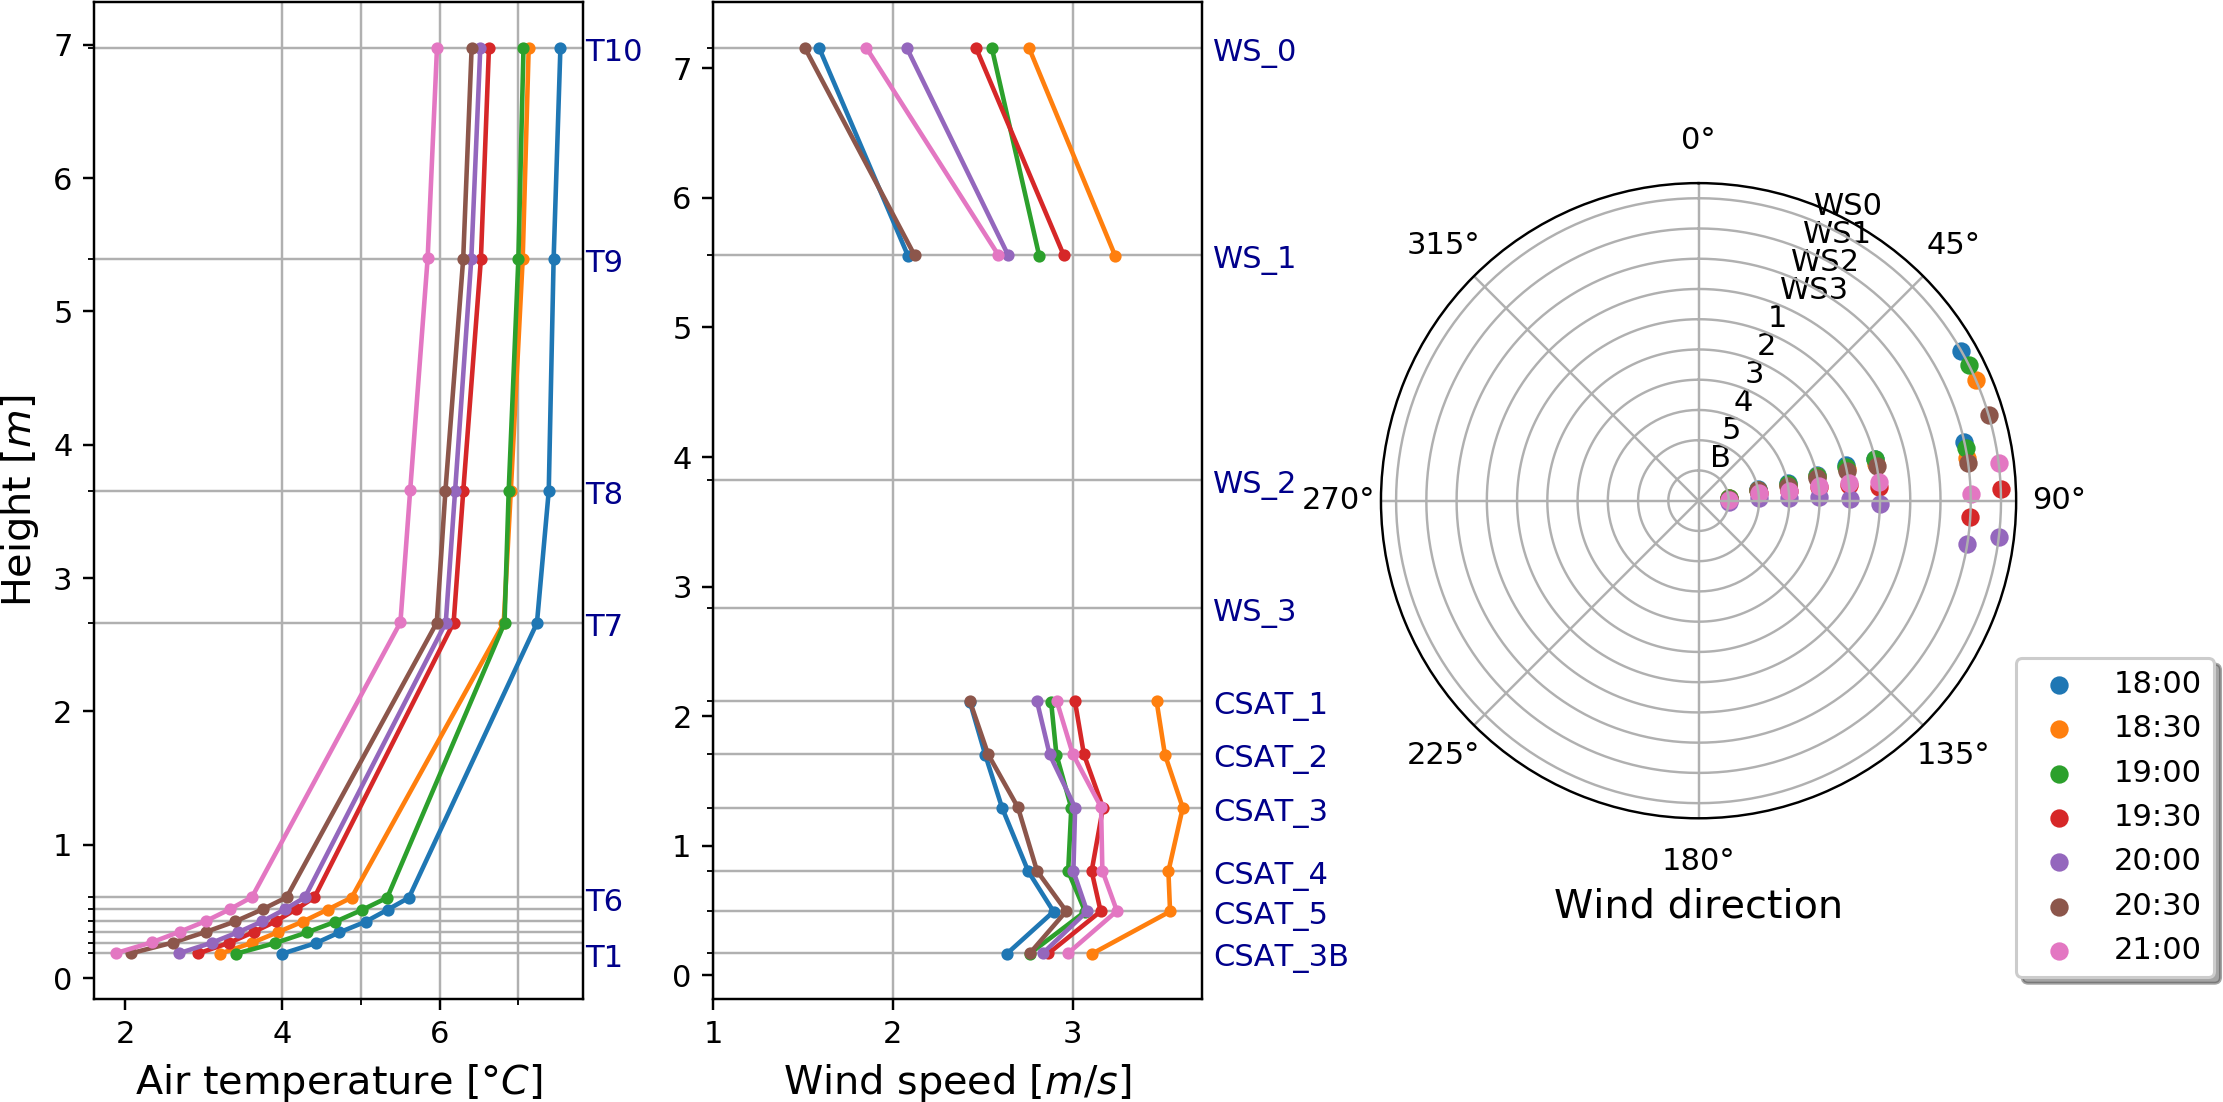
\includegraphics[width=1\textwidth]{fig/chapter_4/16-17/18-21_profiles.png}
    \caption{Temperature and wind speed vertical profiles, with the corresponding wind direction at a particular time, for the period between 18h00 and 21h00 on the night of the 16-17th.}
    \label{fig:16-17_18-21_profiles.png}
\end{figure}

\begin{figure}[!ht]
    \centering
    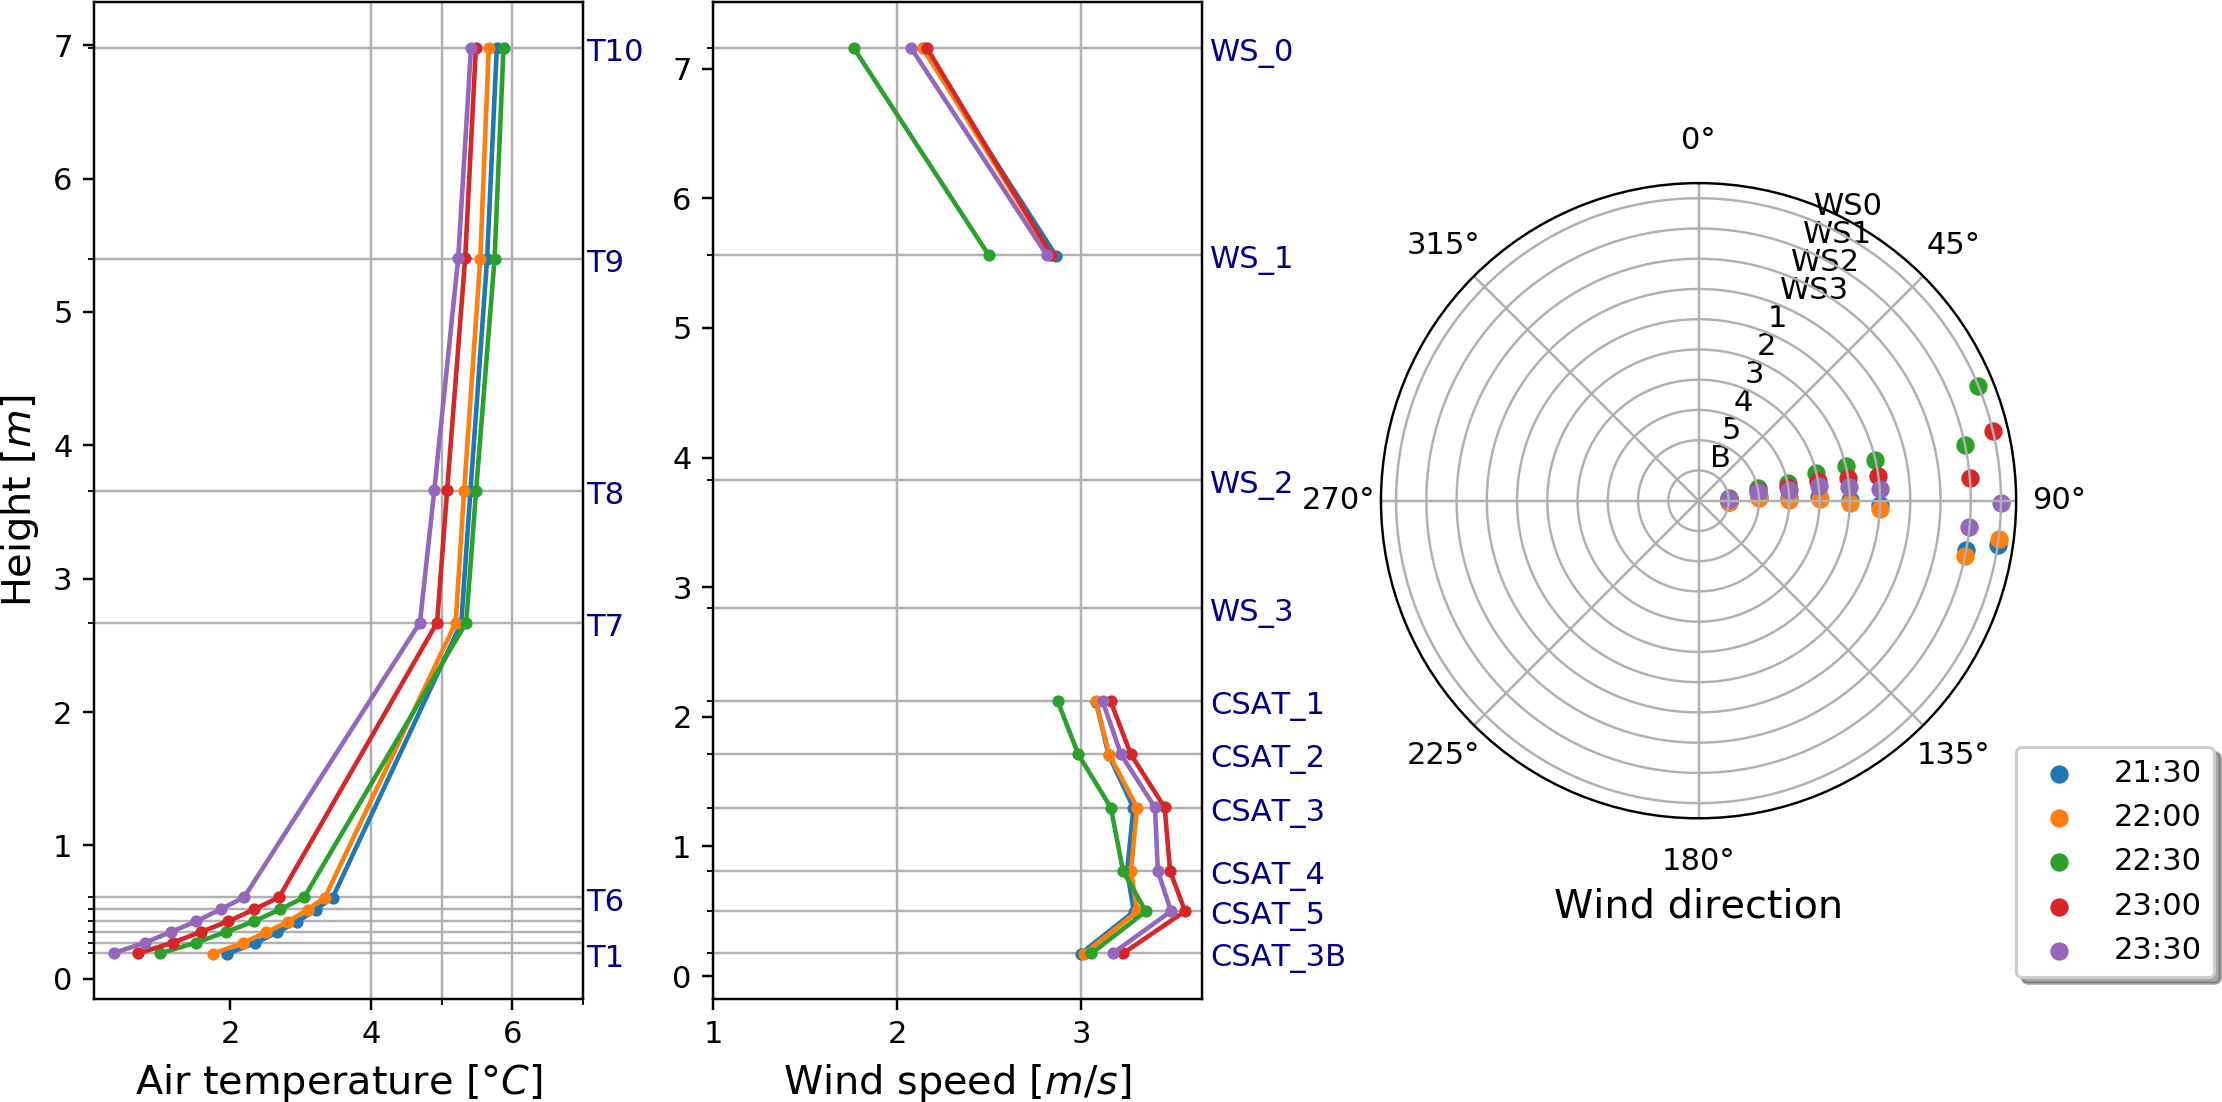
\includegraphics[width=1\textwidth]{fig/chapter_4/16-17/21-23_profiles.png}
    \caption{Temperature and wind speed vertical profiles, with the corresponding wind direction at a particular time, for the period between 21h30 and 23h30 on the night of the 16-17th.}
    \label{fig:16-17_21-23_profiles.png}
\end{figure}

\begin{figure}[!ht]
    \centering
    \begin{subfigure}[b]{0.6\textwidth}
        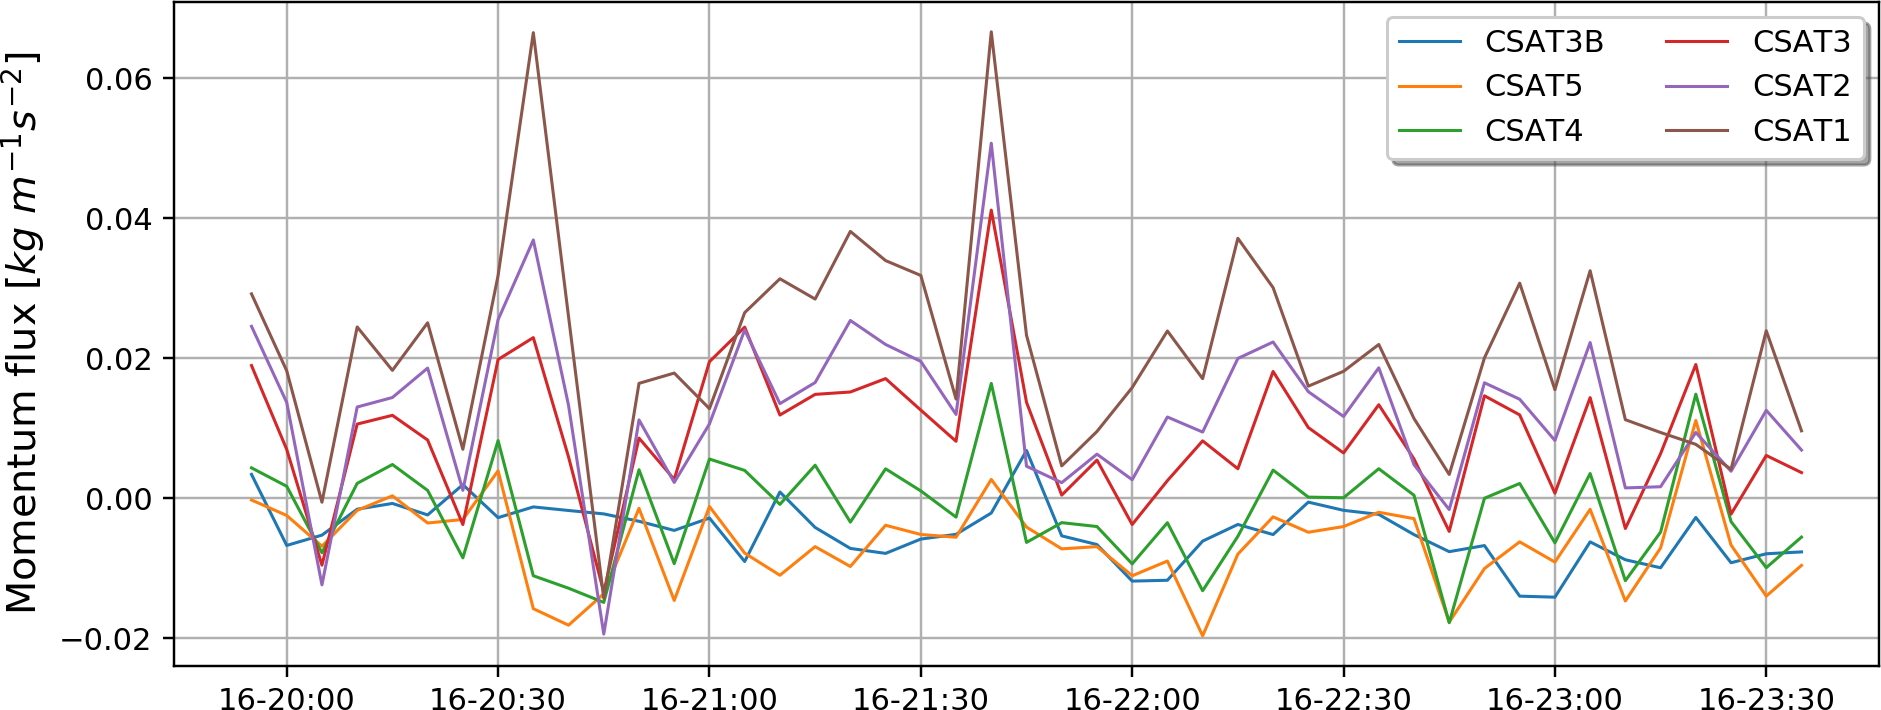
\includegraphics[width=\textwidth]{fig/chapter_4/16-17/Tau_16-17.png}
      \label{fig:Tau_16-17}
    \end{subfigure}
    \begin{subfigure}[b]{0.6\textwidth}
        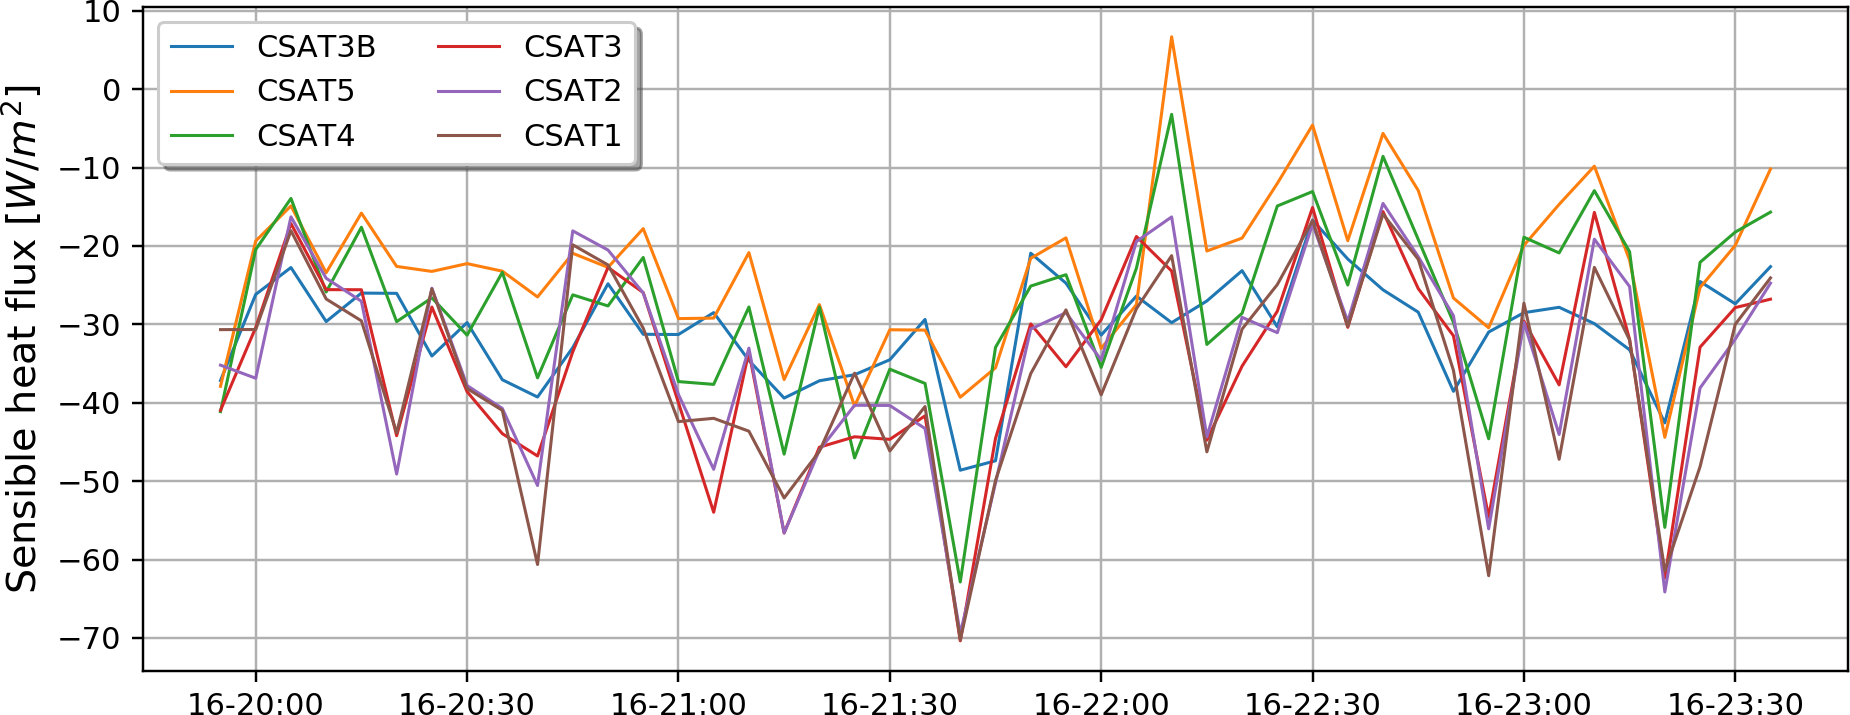
\includegraphics[width=\textwidth]{fig/chapter_4/16-17/H_16-17.png}
        \label{fig:H_16-17}
    \end{subfigure}
    \begin{subfigure}[b]{0.6\textwidth}
        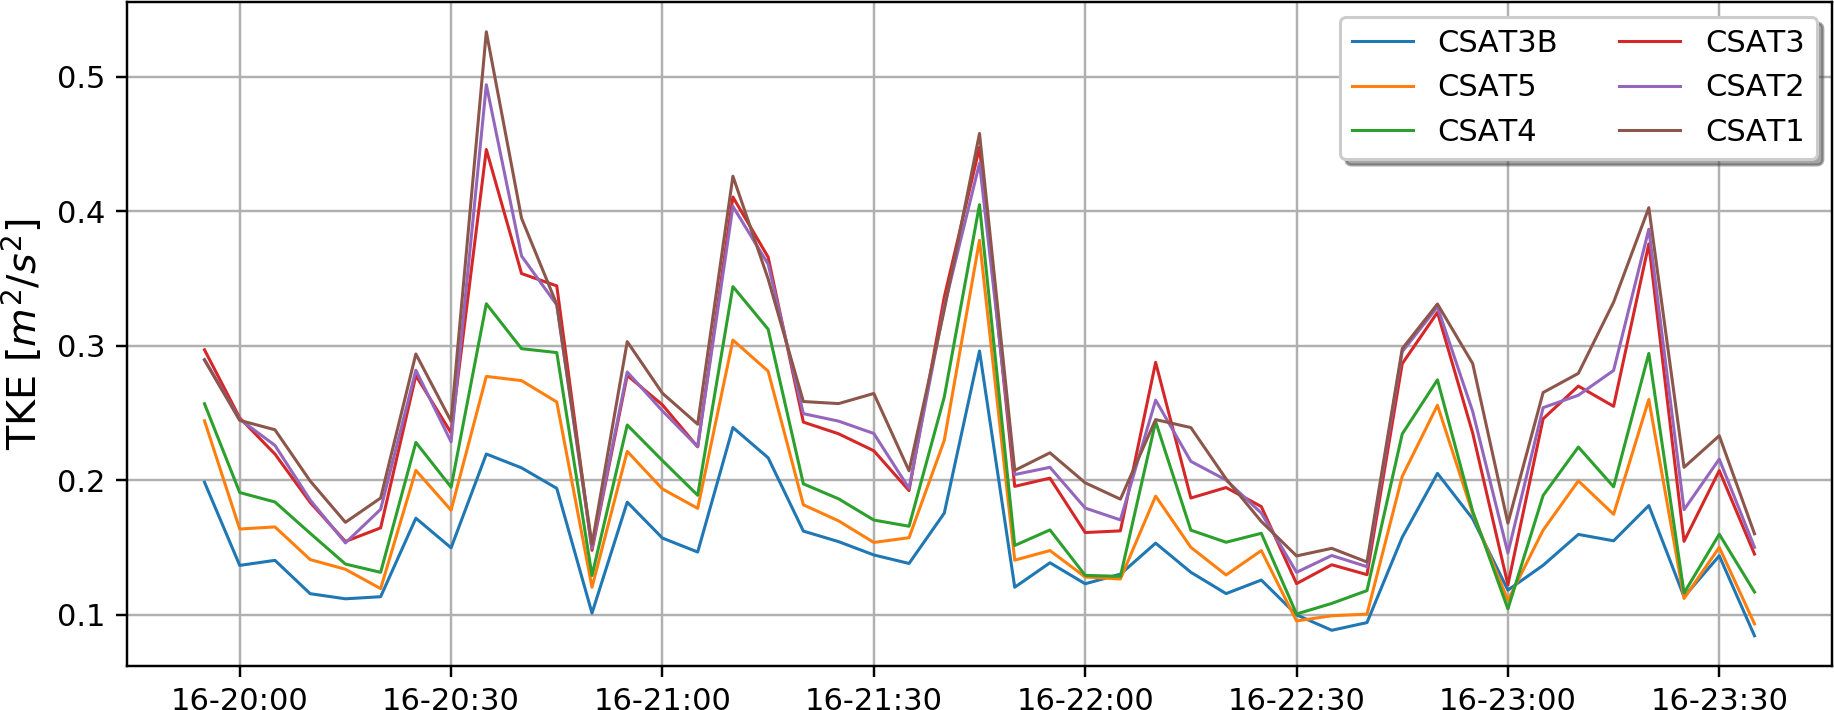
\includegraphics[width=\textwidth]{fig/chapter_4/16-17/TKE_16-17.png}
        \label{fig:TKE_16-17}
    \end{subfigure}
    \caption{Time series of the momentum flux (upper figure), temperature flux (middle figure) and Turbulent Kinetic Energy (lower figure). }
    \label{fig:16-17_flux_series}
\end{figure}
